\documentclass[dvipdfmx,8pt]{beamer}


\usepackage{here, amsmath, latexsym, amssymb, bm, ascmac, mathtools, multicol, tcolorbox, subfig,color}
\usepackage{tikz}
\usepackage{graphicx}
\usepackage{pxjahyper}%しおりの文字化けを防ぐ
\renewcommand{\baselinestretch}{1.2}
\renewcommand{\figurename}{図}
\renewcommand{\tablename}{表}
\renewcommand\mathfamilydefault{\rmdefault}
\setbeamertemplate{navigation symbols}{}

\usetheme{Boadilla}

\title{第4章 \ 発展的なニューラルネットワーク}
\subtitle{4.1 \ 畳み込みニューラルネットワーク}
\author[須賀]{須賀勇貴}
\institute[茨大]{茨城大学理工学研究科}
\date{\today}

\begin{document}

\frame{\maketitle}

  \begin{frame}{はじめに}
    
    近年の深層学習の二枚看板

    \begin{block}{畳み込みニューラルネットワーク(CNN)}
      画像認識に特化したニューラルネットワーク\\
      ex. 画像認識,物体検出
    \end{block}

    \begin{block}{再帰的ニューラルネットワーク (RNN)}
      時系列データの学習に特化したニューラルネットワーク\\
      ex. 音声認識,言語翻訳,気象予報
    \end{block}
    まず,畳み込みニューラルネットワーク(CNN)について説明する.\\
    \begin{itemize}
      \item 説明すること
      \begin{enumerate}
        \item 画像(猫の画像)と特徴(猫の写っている場所)が相関するモデルを考える
        \item 適切なハミルトニアンの構築
        \item 畳み込み演算の導出
      \end{enumerate}
    \end{itemize}

  \end{frame}


  \begin{frame}{4.1.1 畳み込み}
    \begin{equation}
      i \approx I, j \approx J \text{の辺りに猫が写っている確率} \tag{4.1.1}
    \end{equation}
    この場合の最も素朴なハミルトニアン
    \begin{equation}
      H_{J,x}(\{d_{I,J}\}) = -\sum_{IJ}\left( \sum_{ij}d_{IJ}J_{IJ,ij}x_{ij} + d_{IJ}J_{IJ} \right) \tag{4.1.2}
    \end{equation}
    \begin{figure}
      \centering
        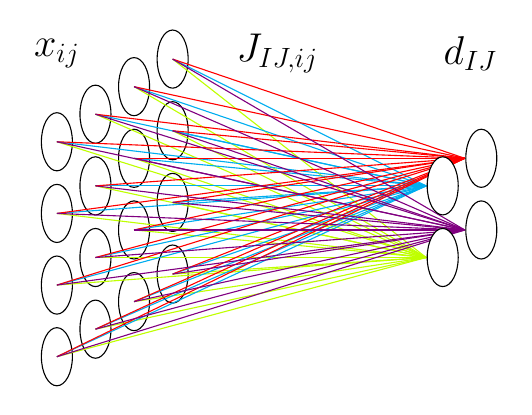
\begin{tikzpicture}[scale=0.7,transform shape]
          \draw (0,0) ellipse (8pt and 15pt);     \draw (0,1.3) ellipse (8pt and 15pt);
          \draw (0,2.6) ellipse (8pt and 15pt);   \draw (0,3.9) ellipse (8pt and 15pt);
          \draw (0.7,0.5) ellipse (8pt and 15pt); \draw (0.7,1.8) ellipse (8pt and 15pt);
          \draw (0.7,3.1) ellipse (8pt and 15pt); \draw (0.7,4.4) ellipse (8pt and 15pt);
          \draw (1.4,1) ellipse (8pt and 15pt);   \draw (1.4,2.3) ellipse (8pt and 15pt);
          \draw (1.4,3.6) ellipse (8pt and 15pt); \draw (1.4,4.9) ellipse (8pt and 15pt);
          \draw (2.1,1.5) ellipse (8pt and 15pt); \draw (2.1,2.8) ellipse (8pt and 15pt);
          \draw (2.1,4.1) ellipse (8pt and 15pt); \draw (2.1,5.4) ellipse (8pt and 15pt);
          \draw [lime] (0  ,0  ) -- (6.7,1.8);    \draw [lime] (0  ,1.3) -- (6.7,1.8);
          \draw [lime] (0  ,2.6) -- (6.7,1.8);    \draw [lime] (0  ,3.9) -- (6.7,1.8);
          \draw [lime] (0.7,0.5) -- (6.7,1.8);    \draw [lime] (0.7,1.8) -- (6.7,1.8);
          \draw [lime] (0.7,3.1) -- (6.7,1.8);    \draw [lime] (0.7,4.4) -- (6.7,1.8);
          \draw [lime] (1.4,1  ) -- (6.7,1.8);    \draw [lime] (1.4,2.3) -- (6.7,1.8);
          \draw [lime] (1.4,3.6) -- (6.7,1.8);    \draw [lime] (1.4,4.9) -- (6.7,1.8);
          \draw [lime] (2.1,1.5) -- (6.7,1.8);    \draw [lime] (2.1,2.8) -- (6.7,1.8);
          \draw [lime] (2.1,4.1) -- (6.7,1.8);    \draw [lime] (2.1,5.4) -- (6.7,1.8);
          \draw [cyan] (0  ,0  ) -- (6.7,3.1);    \draw [cyan] (0  ,1.3) -- (6.7,3.1);
          \draw [cyan] (0  ,2.6) -- (6.7,3.1);    \draw [cyan] (0  ,3.9) -- (6.7,3.1);
          \draw [cyan] (0.7,0.5) -- (6.7,3.1);    \draw [cyan] (0.7,1.8) -- (6.7,3.1);
          \draw [cyan] (0.7,3.1) -- (6.7,3.1);    \draw [cyan] (0.7,4.4) -- (6.7,3.1);
          \draw [cyan] (1.4,1  ) -- (6.7,3.1);    \draw [cyan] (1.4,2.3) -- (6.7,3.1);
          \draw [cyan] (1.4,3.6) -- (6.7,3.1);    \draw [cyan] (1.4,4.9) -- (6.7,3.1);
          \draw [cyan] (2.1,1.5) -- (6.7,3.1);    \draw [cyan] (2.1,2.8) -- (6.7,3.1);
          \draw [cyan] (2.1,4.1) -- (6.7,3.1);    \draw [cyan] (2.1,5.4) -- (6.7,3.1);
          \draw [red] (0  ,0  ) -- (7.4,3.6);     \draw [red] (0  ,1.3) -- (7.4,3.6);
          \draw [red] (0  ,2.6) -- (7.4,3.6);     \draw [red] (0  ,3.9) -- (7.4,3.6);
          \draw [red] (0.7,0.5) -- (7.4,3.6);     \draw [red] (0.7,1.8) -- (7.4,3.6);
          \draw [red] (0.7,3.1) -- (7.4,3.6);     \draw [red] (0.7,4.4) -- (7.4,3.6);
          \draw [red] (1.4,1  ) -- (7.4,3.6);     \draw [red] (1.4,2.3) -- (7.4,3.6);
          \draw [red] (1.4,3.6) -- (7.4,3.6);     \draw [red] (1.4,4.9) -- (7.4,3.6);
          \draw [red] (2.1,1.5) -- (7.4,3.6);     \draw [red] (2.1,2.8) -- (7.4,3.6);
          \draw [red] (2.1,4.1) -- (7.4,3.6);     \draw [red] (2.1,5.4) -- (7.4,3.6);
          \draw [violet] (0  ,0  ) -- (7.4,2.3);  \draw [violet] (0  ,1.3) -- (7.4,2.3);
          \draw [violet] (0  ,2.6) -- (7.4,2.3);  \draw [violet] (0  ,3.9) -- (7.4,2.3);
          \draw [violet] (0.7,0.5) -- (7.4,2.3);  \draw [violet] (0.7,1.8) -- (7.4,2.3);
          \draw [violet] (0.7,3.1) -- (7.4,2.3);  \draw [violet] (0.7,4.4) -- (7.4,2.3);
          \draw [violet] (1.4,1  ) -- (7.4,2.3);  \draw [violet] (1.4,2.3) -- (7.4,2.3);
          \draw [violet] (1.4,3.6) -- (7.4,2.3);  \draw [violet] (1.4,4.9) -- (7.4,2.3);
          \draw [violet] (2.1,1.5) -- (7.4,2.3);  \draw [violet] (2.1,2.8) -- (7.4,2.3);
          \draw [violet] (2.1,4.1) -- (7.4,2.3);  \draw [violet] (2.1,5.4) -- (7.4,2.3);
          \filldraw [fill=white, draw=black] (7,1.8) ellipse (8pt and 15pt);   \filldraw [fill=white, draw=black] (7,3.1) ellipse (8pt and 15pt);
          \filldraw [fill=white, draw=black] (7.7,2.3) ellipse (8pt and 15pt); \filldraw [fill=white, draw=black] (7.7,3.6) ellipse (8pt and 15pt);
  
          \node (a) at (0,5.5) {{\fontsize{20pt}{20pt}\selectfont$x_{ij}$}};
          \node (a) at (4,5.5) {{\fontsize{20pt}{20pt}\selectfont$J_{IJ,ij}$}};
          \node (a) at (7.5,5.5) {{\fontsize{20pt}{20pt}\selectfont$d_{IJ}$}};
        \end{tikzpicture}
    \end{figure}
  \end{frame}

  \begin{frame}{4.1.1 畳み込み}
    (4.1.1)を議論したい場合,全ての$ij$との相互作用を考えても無駄
    \begin{equation}
      J_{IJ,ij}
      =\begin{cases}
        \text{非ゼロ} &\begin{pmatrix} i = s_1 I + \alpha, \ \alpha \in [-W_1/2,W_1/2]\\ j = s_2 J + \beta, \ \beta \in [W_2/2,W_2/2] \end{pmatrix}\\
        \text{ゼロ}   & \text{その他} \tag{4.1.3}
      \end{cases}
    \end{equation}
    \begin{align*}
      s_{1,2} &: \text{ストライド(stride) ・・・「何ピクセル飛ばし」で特徴を捉えるかのパラメータ}\\
      W_{1,2} &: \text{フィルターサイズ ・・・ どのくらいの大きさの領域で特徴を捉えるかのパラメータ}
    \end{align*}
    これを実現できる結合定数
    \begin{equation}
      J_{IJ,ij} = \sum_{\alpha \beta}J_{IJ,\alpha\beta}\delta_{i,s_1I + \alpha}\delta_{j,s_2J + \beta} \tag{4.1.4}
    \end{equation}
  \end{frame}

  \frame{
    \frametitle{4.1.1 畳み込み}
    \begin{columns}[t]
      \begin{column}{0.5\textwidth}
        \small{
          $s_{1,2} = 3, W_{1,2} = 2$のときを考える(右図)
          \begin{equation*}
            J_{IJ,ij} = \sum_{\alpha,\beta = -1}^{1}J_{IJ,\alpha\beta}\delta_{i,3I+\alpha}\delta_{j,3J+\beta}
          \end{equation*}
          \begin{align*}
            &H_{J,x}(\{ d_{IJ}\})\\
            &= -\sum_{I,J=0}^{1}\left(\sum_{i,j=0}^{3}\sum_{\alpha,\beta=-1}^{1}d_{IJ}J_{IJ,\alpha\beta}\delta_{i,3J+\alpha}\delta_{j,3J+\beta}x_{ij}+d_{IJ}\right)\\
            &= -\sum_{I,J=0}^{1}\sum_{\alpha,\beta=-1}^{1}d_{IJ}J_{IJ,\alpha\beta}x_{3I+\alpha,3J+\beta} - \sum_{I,J=0}^{1}d_{IJ}J_{IJ}
          \end{align*}
          \begin{align*}
            \text{1項目}
            &=\color{cyan}d_{00}J_{00,00}x_{00}+ d_{00}J_{00,01}x_{01} + d_{00}J_{00,10}x_{10} + d_{00}J_{00,11}x_{11}\\
            &=\color{red}d_{01}J_{01,02}x_{02}+ d_{01}J_{01,03}x_{03} + d_{01}J_{01,12}x_{12} + d_{01}J_{01,13}x_{13}\\
            &=\color{green}d_{10}J_{10,20}x_{20} + d_{10}J_{10,21}x_{21} + d_{10}J_{10,30}x_{30} + d_{10}J_{10,31}x_{31}\\
            &=\color{violet}d_{11}J_{11,22}x_{22} + d_{11}J_{11,23}x_{23} + d_{11}J_{11,32}x_{32} +d_{11}J_{11,33}x_{33}
          \end{align*}
        }
      \end{column}
      \begin{column}{0.3\textwidth} 
        \begin{figure}
          \begin{center}
            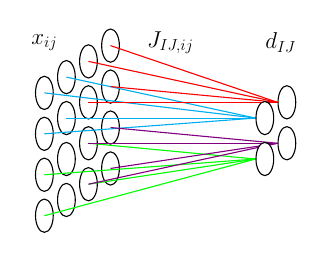
\begin{tikzpicture}[scale=0.4,transform shape]
              \draw (0  ,0  ) ellipse (8pt and 15pt); \draw (0  ,1.3) ellipse (8pt and 15pt);
              \draw (0  ,2.6) ellipse (8pt and 15pt); \draw (0  ,3.9) ellipse (8pt and 15pt);
              \draw (0.7,0.5) ellipse (8pt and 15pt); \draw (0.7,1.8) ellipse (8pt and 15pt);
              \draw (0.7,3.1) ellipse (8pt and 15pt); \draw (0.7,4.4) ellipse (8pt and 15pt);
              \draw (1.4,1  ) ellipse (8pt and 15pt); \draw (1.4,2.3) ellipse (8pt and 15pt);
              \draw (1.4,3.6) ellipse (8pt and 15pt); \draw (1.4,4.9) ellipse (8pt and 15pt);
              \draw (2.1,1.5) ellipse (8pt and 15pt); \draw (2.1,2.8) ellipse (8pt and 15pt);
              \draw (2.1,4.1) ellipse (8pt and 15pt); \draw (2.1,5.4) ellipse (8pt and 15pt);
            
              \draw [green] (0,0  ) -- (6.7,1.8);  \draw [green] (0  ,1.3) -- (6.7,1.8);
              \draw [green] (1.4,1) -- (6.7,1.8);  \draw [green] (1.4,2.3) -- (6.7,1.8);
              \draw [cyan] (0  ,2.6) -- (6.7,3.1);\draw [cyan] (0  ,3.9) -- (6.7,3.1);
              \draw [cyan] (0.7,3.1) -- (6.7,3.1);\draw [cyan] (0.7,4.4) -- (6.7,3.1);
              \draw [red] (1.4,3.6) -- (7.4,3.6);\draw [red] (1.4,4.9) -- (7.4,3.6);
              \draw [red] (2.1,4.1) -- (7.4,3.6);\draw [red] (2.1,5.4) -- (7.4,3.6);
              \draw [violet] (1.4,1  ) -- (7.4,2.3);\draw [violet] (1.4,2.3) -- (7.4,2.3);
              \draw [violet] (2.1,1.5) -- (7.4,2.3);\draw [violet] (2.1,2.8) -- (7.4,2.3);
              \filldraw [fill=white, draw=black] (7  ,1.8) ellipse (8pt and 15pt); \filldraw [fill=white, draw=black] (7,3.1) ellipse (8pt and 15pt);
              \filldraw [fill=white, draw=black] (7.7,2.3) ellipse (8pt and 15pt); \filldraw [fill=white, draw=black] (7.7,3.6) ellipse (8pt and 15pt);
            
              \node (a) at (0,5.5) {{\fontsize{20pt}{20pt}\selectfont$x_{ij}$}};
              \node (a) at (4,5.5) {{\fontsize{20pt}{20pt}\selectfont$J_{IJ,ij}$}};
              \node (a) at (7.5,5.5) {{\fontsize{20pt}{20pt}\selectfont$d_{IJ}$}};
            \end{tikzpicture}
            \caption{結合定数の模式図}
          \end{center}   
        \end{figure}
        \begin{align*}
          i,j &= 0,1,2,3 \\ 
          I,J &= 0,1 
        \end{align*}
      \end{column}
    \end{columns}
  }

  \begin{frame}{4.1.1 畳み込み}
    \begin{columns}[t]
      \begin{column}{0.5\textwidth}
        \small{
          猫の写っている場所は真ん中だったり,右側だったりする\\
          \begin{center}
            $\Downarrow$
          \end{center}
          捉えたい画像の特徴が「猫っぽさ」である場合,\\
          その特徴は$I,J$に依存しないはず\\
          \begin{center}
            $\Downarrow$
          \end{center}
          結合定数に$IJ$依存性は入れないことにする
          \begin{equation}
            J_{IJ,ij} = \sum_{\alpha\beta}J_{\alpha\beta}\delta_{i,S_1I+\alpha}\delta_{j,s_2J+\beta} \tag{4.1.5}
          \end{equation}
          ハミルトニアンは
          \begin{align}
            &H_{J,x}^{\text{conv}}(\{d_{IJ}\}) \notag\\
            &= -\sum_{\{d_{IJ}\}}\exp\left[\sum_{IJ}d_{IJ}\left(\sum_{\alpha\beta}J_{\alpha\beta}x_{s_1I+\alpha,s_2J+\beta}+J\right)\right] \tag{4.1.6}
          \end{align}
        }
      \end{column}
      \begin{column}{0.3\textwidth} 
        \begin{figure}
          \begin{center}
            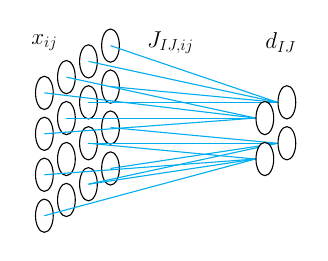
\begin{tikzpicture}[scale=0.4,transform shape]
              \draw (0  ,0  ) ellipse (8pt and 15pt); \draw (0  ,1.3) ellipse (8pt and 15pt);
              \draw (0  ,2.6) ellipse (8pt and 15pt); \draw (0  ,3.9) ellipse (8pt and 15pt);
              \draw (0.7,0.5) ellipse (8pt and 15pt); \draw (0.7,1.8) ellipse (8pt and 15pt);
              \draw (0.7,3.1) ellipse (8pt and 15pt); \draw (0.7,4.4) ellipse (8pt and 15pt);
              \draw (1.4,1  ) ellipse (8pt and 15pt); \draw (1.4,2.3) ellipse (8pt and 15pt);
              \draw (1.4,3.6) ellipse (8pt and 15pt); \draw (1.4,4.9) ellipse (8pt and 15pt);
              \draw (2.1,1.5) ellipse (8pt and 15pt); \draw (2.1,2.8) ellipse (8pt and 15pt);
              \draw (2.1,4.1) ellipse (8pt and 15pt); \draw (2.1,5.4) ellipse (8pt and 15pt);
            
              \draw [cyan] (0,0  ) -- (6.7,1.8);  \draw [cyan] (0  ,1.3) -- (6.7,1.8);
              \draw [cyan] (1.4,1) -- (6.7,1.8);  \draw [cyan] (1.4,2.3) -- (6.7,1.8);
              \draw [cyan] (0  ,2.6) -- (6.7,3.1);\draw [cyan] (0  ,3.9) -- (6.7,3.1);
              \draw [cyan] (0.7,3.1) -- (6.7,3.1);\draw [cyan] (0.7,4.4) -- (6.7,3.1);
              \draw [cyan] (1.4,3.6) -- (7.4,3.6);\draw [cyan] (1.4,4.9) -- (7.4,3.6);
              \draw [cyan] (2.1,4.1) -- (7.4,3.6);\draw [cyan] (2.1,5.4) -- (7.4,3.6);
              \draw [cyan] (1.4,1  ) -- (7.4,2.3);\draw [cyan] (1.4,2.3) -- (7.4,2.3);
              \draw [cyan] (2.1,1.5) -- (7.4,2.3);\draw [cyan] (2.1,2.8) -- (7.4,2.3);
              \filldraw [fill=white, draw=black] (7  ,1.8) ellipse (8pt and 15pt); \filldraw [fill=white, draw=black] (7,3.1) ellipse (8pt and 15pt);
              \filldraw [fill=white, draw=black] (7.7,2.3) ellipse (8pt and 15pt); \filldraw [fill=white, draw=black] (7.7,3.6) ellipse (8pt and 15pt);
            
              \node (a) at (0,5.5) {{\fontsize{20pt}{20pt}\selectfont$x_{ij}$}};
              \node (a) at (4,5.5) {{\fontsize{20pt}{20pt}\selectfont$J_{IJ,ij}$}};
              \node (a) at (7.5,5.5) {{\fontsize{20pt}{20pt}\selectfont$d_{IJ}$}};
            \end{tikzpicture}
            \caption{結合定数の模式図}
          \end{center}   
        \end{figure}
        \begin{align*}
          i,j &= 0,1,2,3 \\ 
          I,J &= 0,1 
        \end{align*}
      \end{column}
    \end{columns}
  \end{frame}

  \begin{frame}{4.1.1 畳み込み}
    \begin{equation*}
      H_{J,x}^{\text{conv}}(\{d_{IJ}\}) = -\sum_{\{d_{IJ}\}}\exp\left[\sum_{IJ}d_{IJ}\left(\sum_{\alpha\beta}J_{\alpha\beta}x_{s_1I+\alpha,s_2J+\beta}+J\right)\right] \tag{4.1.6}
    \end{equation*}
    この状態のボルツマン重みを計算
    \begin{align}
      Q_J(\{d_{IJ}=1|x\})
      &=\frac{\exp\left[-H_{J,x}^{\text{conv}}(\{d_{IJ}=1\})\right]}{\sum_{\{d_{IJ}\}}\exp\left[-H_{J,x}^{\text{conv}}(\{d_{IJ}\})\right]}\notag\\
      &=\frac{\exp\left[\sum_{\alpha\beta}J_{\alpha\beta}x_{s_1I+\alpha,s_2J+\beta}+J\right]}{\sum_{\{d_{IJ}\}}\exp\left[\sum_{IJ}d_{IJ}\left(\sum_{\alpha\beta}J_{\alpha\beta}x_{s_1I+\alpha,s_2J+\beta}+J\right)\right]}\notag\\
      &= \sigma\left(\sum_{\alpha\beta}J_{\alpha\beta}x_{s_1I+\alpha,s_2J+\beta}+J\right) \tag{4.1.7}
    \end{align}
    ここで,
    \begin{equation*}
      \{d_{IJ}\}=
      \begin{pmatrix}
        1&0\\0&0\\
      \end{pmatrix}
      \begin{pmatrix}
        0&1\\0&0\\
      \end{pmatrix}
      \begin{pmatrix}
        0&0\\1&0\\
      \end{pmatrix}
      \begin{pmatrix}
        0&0\\0&1\\
      \end{pmatrix}
    \end{equation*}
  \end{frame}

  \begin{frame}{4.1.1 畳み込み}
    \begin{equation*}
      Q_J(\{d_{IJ}=1|x\})
      = \sigma\left(\sum_{\alpha\beta}J_{\alpha\beta}x_{s_1I+\alpha,s_2J+\beta}+J\right) \tag{4.1.7}
    \end{equation*}
    このときの演算
    \begin{equation}
      x_{ij} \rightarrow \sum_{\alpha\beta}J_{\alpha\beta}x_{x_{s_1I+\alpha,s_2J+\beta}} \tag{4.1.8}
    \end{equation}
    を畳み込み演算という\\
    \vspace{0.3cm}
    \begin{center}
    畳み込み演算を含むニューラルネットワーク $\rightarrow$ 畳み込みニューラルネットワーク
    \end{center}
    \vspace{0.3cm}
    現在,画像認識において畳み込みニューラルネットワークは常識となっている
  \end{frame}

  \begin{frame}{4.1.2 転置畳み込み}


  \end{frame}




\end{document}